\documentclass[10pt,twocolumn,letterpaper]{article}

\usepackage{iccv}
\usepackage{times}
\usepackage{epsfig}
\usepackage{graphicx}
\usepackage{amsmath}
\usepackage{amssymb}
\usepackage[numbers,compress]{natbib}
\usepackage{booktabs}

% Include other packages here, before hyperref.

% If you comment hyperref and then uncomment it, you should delete
% egpaper.aux before re-running latex.  (Or just hit 'q' on the first latex
% run, let it finish, and you should be clear).
\usepackage[pagebackref=true,breaklinks=true,letterpaper=true,colorlinks,bookmarks=false,colorlinks=true,allcolors=blue]{hyperref}


 \iccvfinalcopy % *** Uncomment this line for the final submission

% Pages are numbered in submission mode, and unnumbered in camera-ready
\ificcvfinal\pagestyle{empty}\fi

\begin{document}

%%%%%%%%% TITLE
\title{UCF CAP 5516 Project Proposal}

\author{Ronald Campos\\
MSCV Program\\
{\tt\small roncamposj@knights.ucf.edu}
\and
Suneet Tipirneni\\
MSCV Program\\
{\tt\small  suneet.tipirneni@knights.ucf.edu}
}

\maketitle
% Remove page # from the first page of camera-ready.
\ificcvfinal\thispagestyle{empty}\fi


\begin{abstract}
    As healthcare becomes more democratized, the need to validate potential harmful substances has become more and more important. This is especially true when it comes to medications. We want to propose an alternative way to identify pills by developing
    a model for identifying pills that relies on the robust and modern transformer architecture.
\end{abstract}


\section{Problem Definition}
Given an input of an image, our goal is to identity and provide a text output for pills/medications in the image. Having more tools to identify potentially hazardous substances can lead to safer environments especially in the pharmaceutical domain. The end goal of this project is to enable people with a non-pharmaceutical background the ability to identify pills/medications with ease using computer vision.

\section{Related Work}

Our related work is primarily comprised of the existing knowledge of vision transformers and the original paper
that performed pill identification using a CNN-like architecture.
\begin{itemize}
    \item An Image is Worth 16x16 Words: Transformers for Image Recognition at Scale \cite{an_imageworth}
        \item A Low-Shot Fine-Grained Benchmark for Pill Identification \cite{ePill}
\end{itemize}

\section{Dataset}
We will be using the ePillID dataset \cite{ePill} for this work.  This dataset contains $13,000$ images and $4,902$ different pills.  There are $9,804$ different classes in the dataset, as there are two side to each pill.

\section{Method}
% Please add the following required packages to your document preamble:
% \usepackage{booktabs}
We attempt to adapt the model architecture from \cite{ePill}, by using a Transformer encoder in place of the regular embedding layer. The multi-head attention
mechanism of the Transformer encoder should make the model more effective at learning the fine-grained details of the pill images. As such, we see its use for 
Fine-Grained Visual Categorization (FGVC) not only a suitable alternative, but one that could help improve overall performance of these models.

\begin{figure}[h]
    \centering
    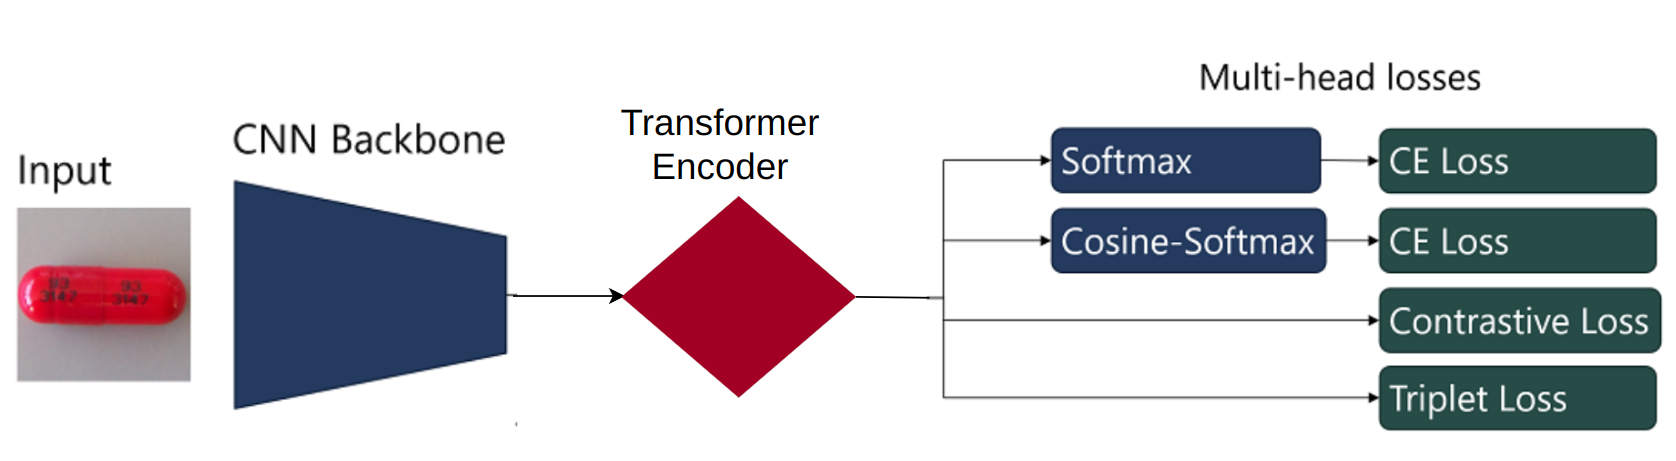
\includegraphics[width=.5\textwidth]{encoder.png}
    \caption{The architecture closely resembles the approach used by \cite{repo}. Instead of only using linear projections
    in an embedding layer, we experiment with adding a Transformer encoder.}
    \label{fig:t_head}
\end{figure}

\subsection{Losses}
The pill images in the dataset are structured in a way that they only ever appear once during training or testing, making this a complicated, few-shot classification task. To remedy this, we employ the multihead-loss implemented in~\cite{ePill}.  The loss is defined by:
\begin{equation}
L_{final} = \lambda_{SCE}L_{SCE} + \lambda_\eta L_\eta + \lambda_\rho L_\rho + \lambda_\Gamma L_\Gamma,
\end{equation}
where $L_{SCE}$ is a standard softmax cross-entropy loss, $L_\eta$ the arcface loss \cite{arc}, $L_\rho$ the triplet loss \cite{triplet}, and $L_\Gamma$ the contrastive loss \cite{contrast}. 
$\lambda$, $\lambda_\eta$, $\lambda_\rho$, $\lambda_\Gamma$ are just weights for the losses. The definitions of these are as follows:



\subsubsection{Arcface Loss}
\begin{equation}
L_\eta = -\log \frac{e^{s\cdot \text{cos}(\theta_{y_i})}}{e^{s\cdot \text{cos}(\theta_{y_i})} + \sum_{j=1, j\neq y_i}^N e^{s\cdot \text{cos}(\theta_j)}},
\end{equation}
where $\theta_{yi}$ is the angle between the weight vector $W_j$ of the true class $y_i$, and the feature $x_i$. $s$ is a scaling factor. The goal of $L_\eta$ is to maximize 
the margin and provide confidence scores between different classes.
\subsubsection{Triplet Loss}
\begin{equation}
    L_\rho = \sum_{i=1}^{N}\left[\left||f\left(x_{i}^{a}\right)-f\left(x_{i}^{p}\right)\right||_{2}^{2}-\left||f\left(x_{i}^{a}\right)-f\left(x_{i}^{n}\right)\right||_{2}^{2}+\alpha\right]_{+},
\end{equation}
where $x_i^a$, $x_i^p$, and $x_i^n$ are the respective anchor, positive, and negative samples, and $f(\cdot)$ is an embedding function function. The goal of $L_\rho$ is to create an embedding space where $x_i^a$ and $x_i^p$ are closely related points in that space. Additionally, 
we want to maximize the distance between $x_i^a$ and $x_i^n$ in that space.
\subsubsection{Contrastive Loss}
\begin{equation}
L_\Gamma = \frac{1}{N} \sum_{i=1}^N \max(0, d_{pos} - d_{neg} + margin),
\end{equation}
where $d_{pos}$ are a postive examples, and $d_{neg}$ negative ones. With $L_\Gamma$, we take $d_{pos}$ and $d_{neg}$ as sample pairs, and our aim is to create a margin between the two sets of classes.

\subsection{Multi-Head Model}
In order to implement the triplet and contrastive losses, we need to add additional overhead to our embedded transformer architecture. 
To compare these two, we use the binary classifier head from \cite{repo} and pass the output $emb$ from the embedded model.  In the case of the arcface loss, a margin head is used in parallel, which also takes $emb$ as input, along with the target values.

\section{Experiments}

    
Our best performing model is trained for 70 epochs and uses pretrained weights, trained on the original ePill architecture for 300 epochs. We train with a batch size of 48, 
and with an initial learning rate of $0.0001$. We also employ a learning rate scheduler, which decreases the learning rate by a factor of $0.5$ 
every time there is a plateau in the GAP score. The values for $\lambda$, $\lambda_\eta$, $\lambda_\rho$, and $\lambda_\Gamma$ are $1.0,0.1,1.0$ and $1.0$ 
respectively. These were empirically tested by \cite{ePill} and still used here. We experimented with a variation of transformer heads and encoder layers and found that the best
performance resulted when we used 4 transformer heads and 2 encoder layers.
Our experiments were conducted with either an Nvidia V100 or Nvidia RTX 3080 Ti GPU.

\subsubsection{Unsuccessful Experiments}\label{sec:failed}
Originally, our goal was to use a Transformer backbone in place of a CNN. We attempted to train our data using a ViT base-16 Transformer \cite{an_imageworth} 
as the replacement for the CNN. We quickly found that our data was too small in size for an architecture of this nature, and shifted to a Swin v2 Tiny Transformer 
\cite{swinv2}. After training with many different configurations, we found that the Swin v2 Tiny Transformer was not able to outperform the CNN backbone. We believe 
this is due to the fact that the Swin v2 Tiny Transformer may not excel at learning local features in a few-shot setting, to the extent that CNNs like ResNet50
or VGG would. 


\section{Results}

Let us review that global average precision (GAP) represents the performances in both precision and recall of a classifier as a single metric. The mean average precision 
(MAP) is the average of the average precision scores for each class. The GAP@1 and MAP@1 metrics represent the top 1 predictions. 
\\

The results shown in Table \ref{tab:results} show that when
compared to the original proposed architecture, we outperform the model in both GAP metrics when employing a Transformer encoder in our embedding layer. Our configuration
allows us to obtain a GAP score that is over 4\% higher and GAP@1 is over 6\% better. This improvement is likely due to the fact that the Transformer encoder is able to
learn more complex relationships between the anchor and positive images, and thus is able to better compute the losses, resulting in better precision and recall scores. 

% The reason our extra layer of embedding improves learning, is likely due to the nature of the problem.  The embedding layer is comprised of two linear layers, 
% one batch normalization layer after the first linear layer, a ReLU operation, and a final tanh activation. The non-linearity from this tanh activation allows 
% us to model the complex relationship between anchor and positive images, helping us with computing our losses. 

\begin{table}[h]
    \caption{* denotes the use of a pretrained model.  + denotes models which have an extra embedding layer added to the transformer output.}

    \begin{tabular}{|ccccc|}
    \hline
    \multicolumn{1}{|c|}{Model}       & \multicolumn{1}{c|}{GAP}   & \multicolumn{1}{c|}{GAP@1} & \multicolumn{1}{c|}{MAP}   & MAP@1 \\ \hline
    \multicolumn{5}{|c|}{\textbf{Multi-head Metric Learning: Both-sides input}}                                                      \\ \hline
    \multicolumn{1}{|c|}{ResNet50}    & \multicolumn{1}{c|}{58.75} & \multicolumn{1}{c|}{80.26} & \multicolumn{1}{c|}{83.51} & 74.28 \\ \hline
    \multicolumn{1}{|c|}{Swin\_v2 *+} & \multicolumn{1}{c|}{46.83} & \multicolumn{1}{c|}{71.54} & \multicolumn{1}{c|}{77.05} & 65.18 \\ \hline
    \multicolumn{1}{|c|}{Swin\_v2 +}  & \multicolumn{1}{c|}{7.73}  & \multicolumn{1}{c|}{32.45} & \multicolumn{1}{c|}{28.67} & 15.65 \\ \hline
    \multicolumn{1}{|c|}{Ours *+}   & \multicolumn{1}{c|}{\textbf{62.96}} & \multicolumn{1}{c|}{\textbf{86.59}} & \multicolumn{1}{c|}{83.56} & 73.96 \\ \hline
    \end{tabular}
    \label{tab:results}
\end{table}
We can see from our results in Figure \ref{fig:loss_graphs} that the triplet, contrastive, and to a lesser extent the arcface loss, all lack stability. 
We believe this is due to the nature few-shot classification, and at the time of writing this paper, using a transformer encoder to embed our features
is our best performing approach. In the future, we would like to look into model-agnostic meta-learning (MAML) \cite{maml} and its variants, as well as 
other few-shot learning methods, to see if these can improve our overall performance.
% the losses for these two are measured similarly.  These both use a binary head classifier that measure euclidian distances between anchor, positive, and 
% negative images (in the cases of the triplet loss). \cite{triplet}\cite{contrast} In the case of arcface, its loss decreased much slower 
% than the rest of the losses, almost in a linear manner. The overall loss began at around $14$ and 
% finished at around $4$. Finding a method which further improves the performance of both the contrastive and triplet
% loss should help improve the overall loss and performance. 

\section{Conclusion}

As shown above we currently achieve what we consider a consistent accuracy for identification. As a result, there are most likely be methods using a completely different assumption that 
can improve the robustness of our apporach.  \par

More specifically, further modifications to the original architecture will be needed. The model as provided make the assumption that a standard embedding layer is an MLP. However, in our case with the transformer, it would be preferable to do some kind of encoding that is specific to the mult-head trainer. Note while vision transformers and SWIN transformers do perform image-specific encoding, they cannot be used directly as per \ref{sec:failed}. We think our solution is a foundation for more work to implemented specific to pill identification.

 \par



{\small
\bibliographystyle{unsrt}
\bibliography{sample}
}

\newpage
\section{Appendix}
\onecolumn
\begin{figure}[h!]
    \begin{tabular}{cc}
        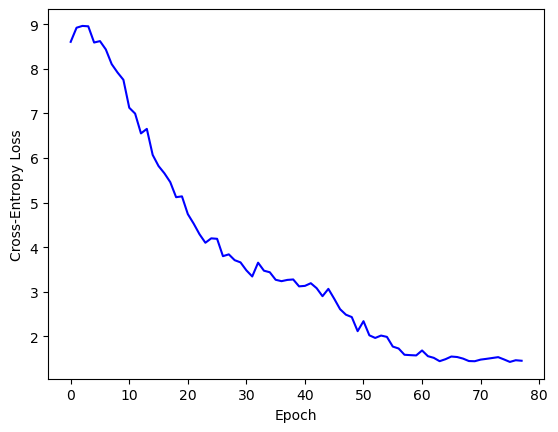
\includegraphics[width=.5\textwidth]{../loss_imgs/ce.png}&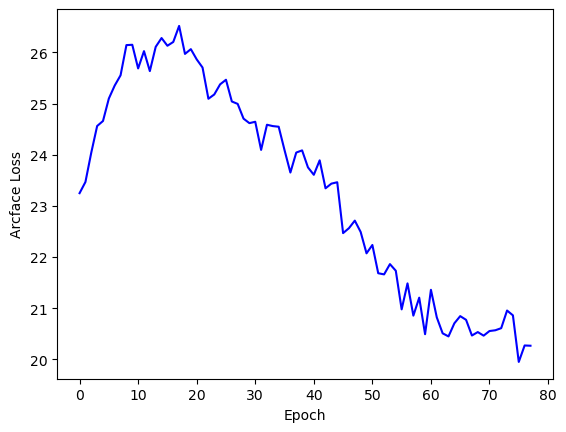
\includegraphics[width=.5\textwidth]{../loss_imgs/arc.png}\\
        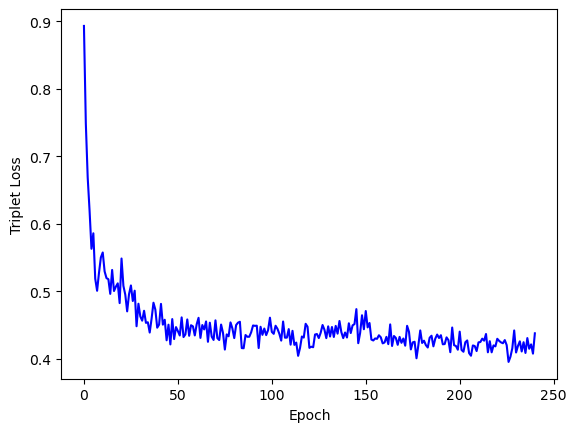
\includegraphics[width=.5\textwidth]{../loss_imgs/triplet.png}&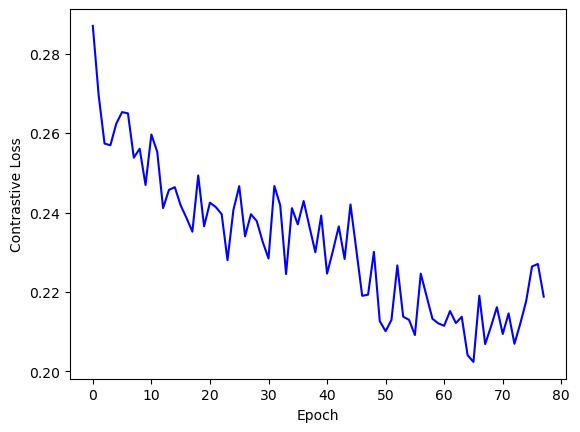
\includegraphics[width=.5\textwidth]{../loss_imgs/cont.png}\\
        \multicolumn{2}{c}{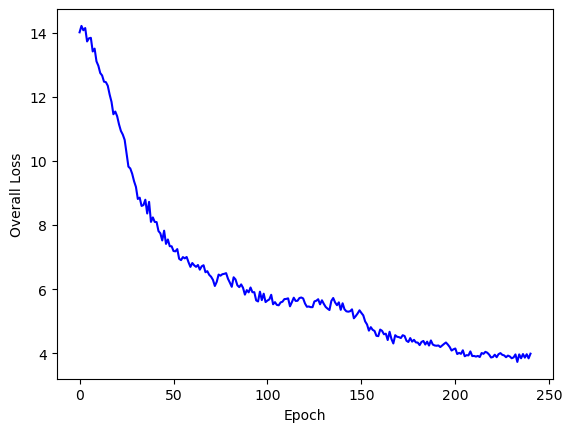
\includegraphics[width=.5\textwidth]{../loss_imgs/overall.png}}
    \end{tabular}
    \caption{The figure shows each of the individual losses from our experiment, as well as their sum (overall loss)}    
    \label{fig:loss_graphs}

\end{figure}
\twocolumn


\end{document}
